% !TeX program = pdflatex
% ISBI 2027 four-page paper. Style files: spconf.sty, IEEEbib.bst.
% Numbers are generated into numbers.tex by scripts/isbi_numbers.py from isbi2027/results_*.json.
% Figures: figures/fig_overview.pdf (scripts/isbi_overview_fig.py), figures/fig_results.pdf (scripts/isbi_figures.py).
% Earlier draft: main_v1_draft.tex.
\documentclass{article}
\usepackage[T1]{fontenc}
\usepackage{spconf,amsmath,amssymb,graphicx}
\usepackage{enumitem}
\usepackage{booktabs}
\usepackage{url}
\usepackage{xcolor}
\setlist{nosep, leftmargin=14pt}
\newcommand{\todo}[1]{\textcolor{red}{[TODO: #1]}}
% generated by scripts/isbi_numbers.py; do not edit
\newcommand{\Nanimals}{52}
\newcommand{\Nsessions}{21}
\newcommand{\Nregions}{31}
\newcommand{\Nsham}{16}
\newcommand{\Ntenpsi}{18}
\newcommand{\Ntwentypsi}{18}
\newcommand{\ICC}{0.18}
\newcommand{\ICCnull}{0.02}
\newcommand{\ICCp}{0.019}
\newcommand{\SDCbefore}{0.84}
\newcommand{\SDCafter}{0.90}
\newcommand{\Motion}{0.7}
\newcommand{\FAnaive}{2/16}
\newcommand{\FAsaccm}{0/14}
\newcommand{\NtestSACCM}{14}
\newcommand{\TableRows}{RAW & naive & 0.056 & 0.091 & 2/16\\
RAW & SACC & 0.042 & 0.091 & 2/16\\
RAW & SACC+M & 0.005 & 0.030 & 0/14\\
RES-A & naive & 0.040 & 0.091 & 2/16\\
RES-A & SACC & 0.030 & 0.079 & 2/16\\
RES-A & SACC+M & 0.005 & 0.037 & 0/14\\
RES-S & naive & 0.069 & 0.115 & 2/16\\
RES-S & SACC & 0.056 & 0.115 & 2/16\\
RES-S & SACC+M & 0.009 & 0.037 & 1/14\\}
\newcommand{\PowerMax}{10\%}
\newcommand{\VoxPowerMax}{12\%}
\newcommand{\SimSensEighty}{2.8\%}
\newcommand{\SimNullTen}{4.0\%}
\newcommand{\SimNullEighty}{13\%}
\newcommand{\MaxProneA}{24.8}
\newcommand{\MaxProneB}{17.6}
\newcommand{\MaxOther}{10.2}
\newcommand{\AppNblast}{36}
\newcommand{\AppFlagged}{2}
\newcommand{\MRSrho}{-0.12}
\newcommand{\MRSp}{0.47}
\newcommand{\MRSn}{37}


\title{When Can Individual Anomaly Maps Be Trusted in Small Preclinical MRI Cohorts?\\Session-Aware Conformal Calibration in a Ferret Blast-Injury Study}

% TODO: confirm author list, order and affiliations with coauthors (copied from the mouse brain-extraction paper).
\name{Tayyab Ali$^{\star}$, Xin Huang$^{\star}$, Miroslaw Janowski$^{\dagger}$, Guanda Qiao$^{\dagger}$, Lei Zhang$^{\star}$}
\address{$^{\star}$ Department of Computer and Information Sciences, Towson University, Towson, MD, USA\\
$^{\dagger}$ Department of Diagnostic Radiology and Nuclear Medicine,\\
University of Maryland School of Medicine, Baltimore, MD, USA}

\begin{document}
\maketitle

\begin{abstract}
Unsupervised normative models promise per-animal anomaly maps in preclinical imaging, and conformal p-values can turn their scores into maps with false-discovery-rate (FDR) control. That guarantee assumes the test animal is exchangeable with the control animals. Small cohorts are scanned in sessions, and the assumption fails. In an in vivo multimodal (T2, diffusion tensor) MRI cohort of \Nanimals{} ferrets scanned in \Nsessions{} sessions after sham or primary blast exposure, region features showed a session intraclass correlation of \ICC{} (permutation $p=\ICCp$). We propose session-aware conformal calibration (SACC): session-level cross-fitting, leave-own-session-out calibration with equal session weights, and Mondrian stratification on recorded acquisition metadata (SACC+M). On held-out sham sessions with raw features, SACC+M reduced per-animal false alarms from \FAnaive{} to \FAsaccm{}. We also show analytically and by simulation that region-level FDR-controlled detection needs far more control sessions than such studies typically include. In this cohort, no reliable individual-level blast effects were found.
\end{abstract}

\begin{keywords}
Conformal prediction, anomaly detection, normative modelling, preclinical MRI, traumatic brain injury
\end{keywords}

\section{Introduction}
\label{sec:intro}
Normative or unsupervised anomaly-detection models learn the appearance of healthy anatomy and flag deviations without lesion labels~\cite{baur2021,marquand2016}. They suit preclinical injury models, where expert lesion annotations rarely exist and injuries can be diffuse. Raw anomaly scores, however, are not calibrated. Conformal p-values provide finite-sample guarantees, and Benjamini--Hochberg (BH) applied to them controls the FDR~\cite{bates2023,bh1995}. Both guarantees rest on exchangeability between the test animal and the calibration controls.

Preclinical cohorts are small, and animals are scanned in sessions. A session shares a day's shim, coil set-up, positioning and handling, and in our data the experimental groups are unevenly spread across sessions. Animal-level calibration then compares a control with other controls from its own session, while an injured animal from a session without controls has no such partner. The calibration is optimistic for exactly the animals of interest. Hierarchical conformal methods address two-level exchangeability~\cite{dunn2023}, and harmonization methods remove batch effects~\cite{fortin2017}, but to our knowledge neither has been examined for calibrated anomaly maps in small preclinical cohorts. Our contributions (Fig.~\ref{fig:overview}) are:
\begin{itemize}
\item A quantification of the session effect in an in vivo multimodal MRI cohort of a gyrencephalic blast-injury model.
\item SACC, and an acquisition-stratified (Mondrian~\cite{vovk2005}) variant, SACC+M, that uses recorded scanner metadata.
\item A p-value floor and a simulation that together state how many control sessions region-level FDR control requires.
\item A candid application to sham, 10\,psi and 20\,psi ferrets at 3 and 7 days.
\end{itemize}

\section{Methods}
\label{sec:methods}

\begin{figure*}[t]
\centering
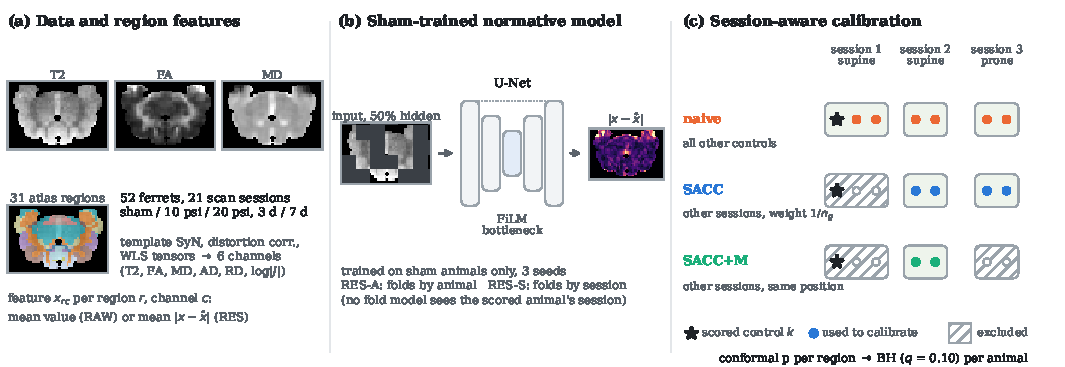
\includegraphics[width=\linewidth]{figures/fig_overview.pdf}
\caption{Overview. (a) T2 and diffusion maps of one sham ferret on the template grid, with the 31 atlas regions used as features. (b) A 2.5D masked autoencoder, trained on sham animals only, reconstructs hidden patches; its absolute error gives residual (RES) features. (c) Calibration of a scored control $k$ (star). The naive scheme calibrates against all other controls, including those scanned in the same session. SACC excludes the scored animal's own session and weights each remaining session equally. SACC+M also excludes sessions with a different recorded position. Conformal p-values per region are then thresholded by BH at $q=0.10$ within each animal.}
\label{fig:overview}
\end{figure*}

\subsection{Data and preprocessing}
We used Bruker 7\,T in vivo scans of \Nanimals{} ferrets: \Nsham{} sham, \Ntenpsi{} at 10\,psi and \Ntwentypsi{} at 20\,psi, at 3 or 7 days after exposure, acquired on \Nsessions{} scan days (sessions). Each scan included axial RARE T2 (0.15$\times$0.15$\times$1.5\,mm), EPI DTI (30 directions, $b=1000/2000$\,s/mm$^2$, 2 repetitions) with a reverse phase-encode $b_0$, and prefrontal PRESS spectroscopy fitted with LCModel~\cite{provencher1993}. Two animals, both scanned in one session, were recorded as prone; all others were supine.

T2 was bias-corrected and registered to an adult ferret template~\cite{hutchinson2017}: rigid atlas transfer, then affine and SyN~\cite{avants2008}. Susceptibility distortion was corrected by a half-way SyN between the forward and reverse $b_0$, restricted to the phase-encode axis, after we found that the vendor's reverse-PE images are stored flipped along that axis (forward/reverse correlation $\approx$0 as stored vs.\ \SDCbefore{} flipped and \SDCafter{} corrected). Motion was corrected rigidly per volume against each $b$-shell mean (maximum \Motion\,mm). Weighted least-squares tensors gave FA, MD, AD and RD. All maps, with the log-Jacobian of the warp, were resampled to the 0.5\,mm template grid. Features are region means over \Nregions{} atlas labels with $\geq$200 voxels in the common field of view (6 channels $\times$ \Nregions{} regions).

\subsection{Normative model}
A 2.5D masked autoencoder~\cite{he2022} (U-Net with a FiLM bottleneck) reconstructs 50\% randomly hidden 8$\times$8 patches across 3 adjacent coronal slices of all 6 channels (Fig.~\ref{fig:overview}b). It is trained on sham animals only, with 3 seeds. Residual features are region means of the absolute reconstruction error. RES-A cross-fits folds by animal; RES-S cross-fits by session, so no fold model sees a control from the scored animal's session.

\subsection{Scores and calibration}
For a test animal $t$ and calibration controls $\mathcal{K}$, the robust z-score per region $r$ and channel $c$ is $z_{rc}=(x_{trc}-\mathrm{med}_\mathcal{K})/(1.4826\,\mathrm{MAD}_\mathcal{K})$, with the scale floored at its 10th percentile. The region score is $s_r=\max_c |z_{rc}|$ for raw features and $\max_c z_{rc}$ for residuals.

The \emph{naive} scheme scores each control against all other controls (leave-one-animal-out). \emph{SACC} scores each control $k$ against controls from \emph{other} sessions only, matching how a test animal from a new session is scored (Fig.~\ref{fig:overview}c). Each calibration session $g$ carries total weight one, split over its $n_g$ animals. The weighted conformal p-value pools region units across sessions:
\begin{equation}
p_r=\frac{1+\sum_{k\in\mathcal{K}}\sum_{r'} w_k\,\mathbb{1}[s^{(k)}_{r'}\geq s_r]}{1+\sum_{k\in\mathcal{K}} w_k\,m},
\label{eq:p}
\end{equation}
with $w_k=1/n_{g(k)}$ and $m$ regions. BH at $q=0.10$ is then applied across the regions of each animal. \emph{SACC+M} restricts $\mathcal{K}$ to controls in the test animal's recorded acquisition stratum (scanner field \texttt{SUBJECT\_\allowbreak position}), a Mondrian split that uses metadata only. Animals whose stratum has fewer than two control sessions are declared not calibratable.

\textbf{A p-value floor.} With $S$ calibration sessions, Eq.~\eqref{eq:p} gives $p_r\geq 1/(1+Sm)$. A single BH rejection needs $p_r\leq q/m$, which is only possible when $S\geq 1/q-1/m$. Even then, the test region must exceed nearly all $Sm$ pooled null scores, so power is governed by the upper tail of the control distribution rather than by the mean shift.

\begin{figure*}[t]
\centering
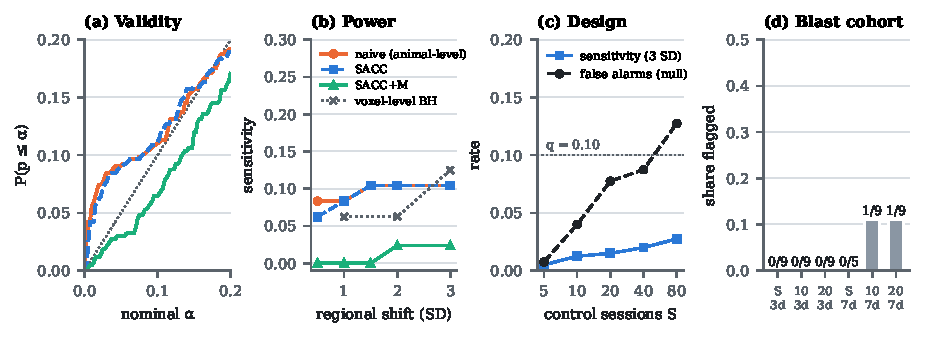
\includegraphics[width=\linewidth]{figures/fig_results.pdf}
\caption{(a) Fraction of p-values $\leq\alpha$ for held-out sham sessions (raw features); the dotted line is nominal. The legend in (b) applies to (a) and (b). (b) Sensitivity to an injected single-region shift (BH $q=0.10$). (c) Simulated sensitivity and null false-alarm rate against the number of control sessions. (d) Animals with $\geq$1 flagged region under SACC+M with raw features (S = sham).}
\label{fig:res}
\end{figure*}

\subsection{Experiments}
The analysis plan was written and hashed before computing results. Two deviations, logged before they were run, added SACC+M and the design simulation.
\begin{enumerate}
\item Session ICC of the raw features after removing group$\times$time means, tested by permuting sessions within cells.
\item Validity for new sessions: each sham session is held out in turn, and its animals are tested against the rest.
\item Semi-synthetic power: a diffuse shift of $a\in\{0.5,\dots,3\}$ between-sham SD is added to one region (FA down; MD, AD, RD and T2 up) in held-out shams. The comparator is voxel-level pooled BH.
\item Design simulation: a Gaussian copula fitted to the supine shams, with session ICC \ICC{} and the empirical heavy-tailed marginals, run for $S\in\{5,\dots,80\}$ sessions.
\item Application to the blast animals.
\end{enumerate}

\section{Results}
\label{sec:results}

\begin{table}[t]
\centering
\caption{New-session validity on held-out sham sessions: fraction of region p-values $\leq\alpha$ (nominal $\alpha$), and shams with $\geq$1 BH-flagged region at $q=0.10$.}
\label{tab:valid}
\small
\setlength{\tabcolsep}{4pt}
\begin{tabular}{@{}llccc@{}}
\toprule
Features & Calibration & $\alpha{=}0.01$ & $\alpha{=}0.05$ & False alarms\\
\midrule
\TableRows
\bottomrule
\end{tabular}
\end{table}

\textbf{Session effect.} The median session ICC of raw region features was \ICC{} (null mean \ICCnull, $p=\ICCp$). The two most extreme controls came from the single prone session (maximum region z of \MaxProneA{} and \MaxProneB{}; all other controls $\leq$\MaxOther).

\textbf{Validity} (Table~\ref{tab:valid}, Fig.~\ref{fig:res}a). Naive and SACC calibration were anti-conservative at small $\alpha$ for raw and session-cross-fitted residual features, and each flagged 2 of 16 held-out shams. SACC+M was at or below nominal, and flagged 0 of \NtestSACCM{} calibratable shams for raw and RES-A features and 1 of \NtestSACCM{} for RES-S. Most of the gain came from excluding the prone session, which reflects heterogeneity that animal-level calibration cannot represent. Session-level cross-fitting of the model (RES-S) did not improve calibration over animal-level cross-fitting (RES-A).

\textbf{Power} (Fig.~\ref{fig:res}b,c). Sensitivity to single-region shifts was at most \PowerMax{} for every scheme up to 3\,SD, and voxel-level BH reached only \VoxPowerMax{} at 3\,SD. In the design simulation, sensitivity at 3\,SD remained \SimSensEighty{} even with $S=80$ control sessions. The null false-alarm rate also rose with $S$ (\SimNullTen{} at $S=10$, \SimNullEighty{} at $S=80$), which shows that pooling across regions is only approximately exchangeable once calibration is precise.

\textbf{Application} (Fig.~\ref{fig:res}d). Under SACC+M, no sham was flagged. Few blast animals were flagged: \AppFlagged{} of \AppNblast{} blast animals, none at 3 days. Prefrontal anomaly evidence was not associated with NAA/tCr (Spearman $\rho=\MRSrho$, $p=\MRSp$, $n=\MRSn$).

\section{Discussion and conclusion}
\label{sec:discussion}
Session clustering and acquisition deviations break the exchangeability on which calibrated anomaly maps rely. Calibrating at the session level, and stratifying by recorded metadata, restores honest false-alarm rates. The price is a sobering power ceiling: with tens of controls, an individual-level, FDR-controlled regional anomaly map can only report changes that exceed nearly all control variability. Calibrated individual maps in small cohorts are therefore best used as a safeguard against over-interpretation, not as a detector.

We recommend that studies record and audit acquisition metadata, spread experimental groups across sessions, scan controls in many sessions rather than many controls per session, and pre-specify a few regions instead of whole-brain voxel or region maps. In this cohort, blast effects detectable in individual animals were not supported. Exploratory group-level regional DTI trends (lower FA, higher MD; not significant after FDR correction) and prior spectroscopy findings~\cite{tang2024} motivate larger, session-balanced designs.

The study has limits. Distortion correction approximates topup~\cite{andersson2003}. Atlas masks were not expert-validated, and registration of the two prone animals was visibly poorer, so their extreme scores reflect acquisition and registration together; SACC+M handles both because it stratifies on the recorded position. Sex and weight were not recorded in the scanner metadata. The SACC+M stratification and the design simulation were added after a first analysis and are disclosed as deviations.

\section{Compliance with ethical standards}
\label{sec:ethics}
\todo{Animal study approval: institution and protocol number (IACUC) for the ferret MRI data, and data-use permission, from coauthors.}

\section{Acknowledgments}
\label{sec:acknowledgments}
\todo{Funding sources; or state that no funding was received.} The authors have no relevant financial or non-financial interests to disclose. An AI assistant (Anthropic Claude) was used to write analysis code, run the analyses and draft this manuscript; the authors reviewed and take responsibility for all content.

\bibliographystyle{IEEEbib}
\bibliography{refs}

\end{document}
